%%%%%%%%%%%%%%%%%%%%%%%%%%%%%%%%%%%%%%%%%%%%%%%%%%%%%%%%%%%%%%%%%%% 
%                                                                 %
%                      THESIS MAIN FILE                           %
%                                                                 %
%%%%%%%%%%%%%%%%%%%%%%%%%%%%%%%%%%%%%%%%%%%%%%%%%%%%%%%%%%%%%%%%%%% 

% document definition 
\documentclass[a4paper,11pt,chap,oneside]{report}

% Use the first command below if you want captions over 1 line indented. A side
% effect of this is to remove the use of bold for captions. To restore bold,
% also include the second line below.

%\usepackage[hang]{caption2}     

% to indent subsequent lines of captions
%\renewcommand{\captionfont}{\bfseries} 
																			 % 
% create the following file in the input from the template
\newcommand{\PaperTitle} {Predicting Object Locations using Spatio-Temporal Information by a Domestic Service Robot: A Bayesian Learning Approach }
\newcommand{\PaperSubject} {Predicting Object Locations using Spatio-Temporal Information by a Domestic Service Robot: A Bayesian Learning Approach}
\newcommand{\PaperTerm} {Summerterm 2016}		
\newcommand{\PaperDate} {\today}			
\newcommand{\ThesisAdvisor} {Dipl. Inform. Tim Niemueller }			
\newcommand{\ThesisReferee} {Prof. Dr. Paul G. Pl\"{o}ger}
\newcommand{\ThesisExReferee} {Prof. Gerhard Lakemeyer, Ph.D.}
\newcommand{\PaperLecturerEMail} {mailto:advisor@xyz}
\newcommand{\Paperkeywords} {key1, key2, key3}		
\newcommand{\PaperMainWriter} {Deebul Nair}
\newcommand{\PaperMainWriterEMail} {mailto:deebul.nair@smail.inf.fh-bonn-rhein-sieg.de}
\newcommand{\ThesisAuthor} {Deebul Nair}
\newcommand{\MatID} {9023573}

%\usepackage[latin1]{inputenc} 

\usepackage{enumitem}
\usepackage[table]{xcolor} 
%\usepackage{graphicx}
\usepackage{color} 
\usepackage{placeins}
\usepackage{transparent} 
\usepackage{hyperref}
\usepackage{tabto}
\usepackage{wrapfig}

\usepackage[draft]{graphicx}
%\usepackage{epstopdf}
\usepackage{url}
%\usepackage[expert,vargreek]{lucidbrb}

%\usepackage{mya4page} % not used, because now is implemented in the class 
\usepackage{amsmath}
%\usepackage{hyperref}
\usepackage{bibnames}
\usepackage{path}
%\usepackage{subfigure}

\usepackage{caption}
\usepackage{subcaption}


\usepackage{amsmath}
\usepackage{todonotes}

\usepackage{tikz}
\usepackage{amsmath}
\usetikzlibrary{bayesnet}
\usepackage{tabularx}
\usepackage{placeins}
\usepackage{pstricks}
\usepackage[titletoc]{appendix}
\usepackage{setspace}


\usepackage[nottoc]{tocbibind}
%\usepackage{footmisc}
%\usepackage[perpage,symbol*]{footmisc} 


%---------------------------------------------------------------
\usepackage{color}
\definecolor{listinggray}{gray}{0.9}
%---------------------------------------------------------------
%\usepackage[copy=false, edit=false]{pdfcrypt}

%---------------------------------------------------------------
\usepackage{listings}
\lstset{language=Java}
\lstset{basicstyle=\footnotesize\small,%ttfamily,%\small,
tabsize=4,
tab=$\to$,
float=tbph,
extendedchars=true,
breaklines,
% prebreak={\space\MyHookSign},
% frame=single,
showtabs=false,
showspaces=false,
showstringspaces=false,
keywordstyle=\color{red}\bfseries,
identifierstyle=\bf\ttfamily,
aboveskip=\bigskipamount,
}
\lstset{captionpos=b}
\lstset{keywordstyle=\color{blue}\bfseries\bf}
\lstset{backgroundcolor=\color{listinggray}, rulecolor=\color{blue}}
\lstset{linewidth=\textwidth}
\lstset{stepnumber=5}
\lstset{numbers=left}
\lstset{numberstyle=\tiny\color{blue}}
\lstset{commentstyle=\color{magenta}\textit, stringstyle=\upshape,
	showstringspaces=false}
\lstset{frame=trBL,frameround=tttt}
%---------------------------------------------------------------

%% Hyperref setup
\usepackage{hyperref}
\hypersetup{
	 a4paper,
   colorlinks=true,
   linkcolor=black,
   filecolor=black,
   citecolor=black,
   urlcolor=black,
   plainpages=false,
   pdftitle={ \PaperTitle },
   pdfsubject={ \PaperSubject },
   pdfauthor={ \ThesisAuthor <deebul.nair@smail.inf.h-brs.de>},
   pdfkeywords={ \Paperkeywords },
   bookmarksnumbered=true,
   pdfpagemode=UseOutlines,
   pdfpagelayout=SinglePage,  
   bookmarksopen=true
}
%\usepackage[copy=true, edit=false, annotate=true]{pdfcrypt}

\usepackage{fancyhdr}
\setlength{\headheight}{15pt}

\pagestyle{fancy}
\renewcommand{\chaptermark}[1]{ \markboth{#1}{} }
\renewcommand{\sectionmark}[1]{ \markright{#1} }

\fancyhf{}
\fancyhead[LE,RO]{\thepage}
\fancyhead[RE]{\textit{ \nouppercase{\leftmark}} }
\fancyhead[LO]{\textit{ \nouppercase{\rightmark}} }

\fancypagestyle{plain}{ %
  \fancyhf{} % remove everything
  \renewcommand{\headrulewidth}{0pt} % remove lines as well
  \renewcommand{\footrulewidth}{0pt}
}
\lstset{
    numbers=none,                
    tabsize=4,
    rulecolor=,
    language=Python,
        basicstyle=\scriptsize,
        upquote=true,
        aboveskip={1.5\baselineskip},
        columns=fixed,
        showstringspaces=false,
        extendedchars=true,
        breaklines=true,
        prebreak = \raisebox{0ex}[0ex][0ex]{\ensuremath{\hookleftarrow}},
        frame=single,
        showtabs=false,
        showspaces=false,
        showstringspaces=false,
        identifierstyle=\ttfamily,
        keywordstyle=\ttfamily
}


\begin{document}
\pagenumbering{gobble}
\begin{titlepage}
\raggedright
\includegraphics[width=0.4\textwidth]{pictures/FH-Header.jpg}\\
\centering
\vspace*{1in}
\begin{Large}\bfseries
\PaperSubject \par
\end{Large}
\vspace{1.2in}
\begin{LARGE}\bfseries
 \par
\end{LARGE}
\vspace{0.5in}
\begin{large}
\PaperMainWriter%\href{\PaperMainWriterEMail}{\PaperMainWriter \footnote{\href{\PaperMainWriterEMail} {santosh.thoduka@smail.inf.fh-bonn-rhein-sieg.de}}}
 \par
\end{large}
\vspace{0.5in}
A thesis submitted in partial fulfilment of the requirements for the degree of
Master of Science in Autonomous Systems \\
at Bonn-Rhein-Sieg University of Applied Sciences
\vfill
\vspace{0.5in}
\par
\vfill
Thesis Supervisors:\\
\ThesisReferee \\ %\href{\PaperLecturerEMail}{\PaperLecturer \footnote{\href{\PaperLecturerEMail} {paul.ploeger@h-brs.de}}}\\
\ThesisExReferee \\ % \href{\SecondSupervisorEMail}{\SecondSupervisor \footnote{\href{\SecondSupervisorEMail} {gerhard.kraetzschmar@h-brs.de}}}\\
\ThesisAdvisor \\
\vspace{0.4in} %\href{\ThirdSupervisorEMail}{\ThirdSupervisor \footnote{\href{\ThirdSupervisorEMail} {frederik.hegger@h-brs.de}}}
September 2016

\end{titlepage}




   
\onehalfspacing
\pagenumbering{roman}

\thispagestyle{empty}
\hbox{}
\vfill
\noindent
I, Deebul Nair Sivarajan, declare that this work has not previously been submitted to this or any other university and that, unless otherwise stated, it is entirely my own work.
\vskip 60pt

\hrule width 2.5cm
\hfill \hspace{5cm}
\hrulefill
\vskip -4pt
\leftline{\hspace{0.6cm} Date \hfill Signature \hspace{1.1cm}}   

\clearpage
%%%%%%%%%%%%%%%%%%%%%%%%%%%%%%%%%%%%%%%%%%%%%%%%%%%%%%%%%%%%%%%%%%% 
%                                                                 %
%                            ABSTRACT                             %
%                                                                 %
%%%%%%%%%%%%%%%%%%%%%%%%%%%%%%%%%%%%%%%%%%%%%%%%%%%%%%%%%%%%%%%%%%% 
\begin{abstract}


In the future, we envison domestic robots to provide useful services both in domestic as well as in industrial context. Examples include domestic service robots, that implements large part of our housework, versatile assistants, that provide automation, transportationm inspection and monitoring services. The challenge in these aplications is that the robots has to have lot of information and knowledge about the user and environment to operate under complete autonomy.This thesis aim is to enable domestic robots to acquire knowledge about behaviour and preferences of the users around them. The developed approaches in this thesis cover the following two topics: (1) learning about the temporal human location behvaiour in-door using previously observed locations of the human (2) learning user preference in object placement. 
 
All techniquies developed in this thesis are based on probabilistic bayesian learning and inference. They have been implemented and evaluated on datasets  collected using real robots as well as on simulated datasets. Extensive experiments have been conducted to evaluate the and validate the properties of the proposed models.
\todo{need to be revised completely}
\end{abstract}
\include{acknowledgement}

\tableofcontents
\listoffigures

\chapter*{Abbreviations}
%\addcontentsline{toc}{chapter}{Abbreviations}
\NumTabs{4}
DCM \tab{Dirichlet Categorical Model}\\
HDCM \tab{Hierarchical Dirichlet Categorical Model}\\
DCBM \tab{Dirichlet Categorical Bernoulli Model}\\
GT \tab{Ground Truth}\\
HMM \tab{Hidden Markov Models}\\
RGB \tab{Red Green Blue} \\
MDP \tab{Markov Decision Process}\\
LCAS \tab{Lincoln Center for Autonomous Systems} \\
CASAS \tab{Center for Advanced Studies in Adaptive Systems}
% the main contents %
\pagenumbering{arabic}
\chapter{Introduction}
\label{chapter:Introduction}

For robots to make a smooth ingress into dynamic human environments like home and office, the robots need to be able to close the \emph{perceive-action-learning} loop. Essentially these domestic service robots should perceive the environment, interact with the environment, learn from experiences and repeat. The robot interacts with the environment by choosing a sequence of low-level actions . For example, lets take the high-level task of ``making coffee", this will require the following actions to be executed sequentially: locate coffee machine, locate coffee pads, locate a cup, place coffee pad in coffee machine, place cup in coffee machine and start coffee machine. But for executing some of the actions like locating the coffee machine, locating the coffee pads, locating the cup etc. the robot needs to have prior knowledge about their possible locations. Such knowledge about the environment and the user needs to be learned by the robot. The goal of this thesis is to enable domestic service robots to gain knowledge about common behaviours and preferences of the user in a non-intrusive manner. Specifically, we address how Bayesian methods can be used to provide a flexible and computationally efficient structure for acquiring knowledge using limited spatio-temporal information collected by domestic service robots.

Domestic service robots need to have the ability to automatically and quickly adapt to a new environment. Imagine if the robot could learn how the user arranges the breakfast table by looking at the data from previous days. Robots can observe the users lifestyle and provide small insights which the user doesn't even notice. The robots can pass along helpful information to the users, like observing their sleep habits and tell them when they are not having adequate sleeps. By learning how the user interacts with their homes and how they live their lives, robots will be able to provide better services to their users. 


\begin{figure}[htp]
\centering
\begin{subfigure}{\textwidth}
  \centering
  \includegraphics[width=\linewidth]{images/introduction.jpg}
\end{subfigure}%
\\
\begin{subfigure}{.24\textwidth}
  \centering
  \includegraphics[width=\linewidth]{images/cup_sink.jpg}
  \caption{cup in sink}
\end{subfigure}
\begin{subfigure}{.24\textwidth}
  \centering
  \includegraphics[width=\linewidth]{images/cup_dishwasher.jpg}
    \caption{cup in dishwasher}
\end{subfigure}
\begin{subfigure}{.24\textwidth}
  \centering
  \includegraphics[width=\linewidth]{images/cup_cupboard.jpg}
    \caption{cup in cupboard}
\end{subfigure}
\begin{subfigure}{.255\textwidth}
  \centering
  \includegraphics[width=\linewidth]{images/robot_view_cup.jpg}
    \caption{cup on table}
\end{subfigure}

\caption[Illustrative example]{Illustrative example of the robot making a record of all the information it has generated in its memory for learning user preferences in object placements}
\end{figure}

Domestic service robots while interacting with the user and environment produce information which after being processed in perception, actuation, or decision making are discarded. \cite{niemueller2012generic} has proposed an approach of storing these information in a robot memory and query the memory for meaningful insights. 
The domestic robot will continuously record sightings of objects and persons with position and time in a database to form the spatio-temporal robot memory. Machine learning is the best method for automatic knowledge generation from the stored information. But in order to adapt quickly the robot needs to able to extract valuable knowledge from small amount of information, i.e., the learning algorithms need to be data efficient.

To illustrate the relevance of the topics presented in this thesis, we motivate our work using a typical task of a domestic service robot.   We assume that the robot is given the task of ``making coffee" for the user, which requires the robot to locate the coffee cup of the user first, make coffee and then to locate the user, for delivering the coffee to him. To begin the search for the coffee cup, it would help the robot to have some prior knowledge about the user's habits; in particular the typical locations where he keeps his cup. This enables the robot to funnel its search for the object from a large number of locations to the most probable ones. Once the coffee cup is located and grasped the robot needs to reason about where it can currently find the user for delivering it to him. This in turn, requires the robot to have knowledge about the likely locations of Waldo at that time.

This motivating example leads us to the two research topics in knowledge acquisition we address in this thesis:
\begin{enumerate}
	\item How can a domestic service robot acquire knowledge about user preferences in placing objects in the environment?
	\item How can a domestic service robot acquire knowledge about the user's temporal location behaviour?
	\item How can a domestic service robot acquire the above knowledge using small amounts of information?
\end{enumerate}

A service robot operating in dynamic human environments needs to perceive the world using its own sensors, and subsequently build a cognitive model of the user preferences and behaviour. These models represent the internal beliefs of the robot about the user preferences and behaviour. The model needs to be extract the knowledge from small amount of information, basically we should develop methods to do data-efficient machine learning. There are many approaches that demonstrate that data-efficient machine learning is possible, including methods like: explicit domain knowledge modelling, exploiting structural knowledge of data, bootstrapping and data augmentation, semi-supervised learning, transfer learning, active learning and Bayesian optimization, non-parametric methods, one-shot learning and Bayesian deep learning \cite{https://sites.google.com/site/dataefficientml/home}. 
Bayesian probabilistic formulation of the cognitive model makes it possible to include the above mentioned methods in a single framework. The robots can use these models to predict the future behaviour of the user or can make educated guess about the user while doing actions with partial information.


In sum, this thesis provides Bayesian probabilistic techniques that enable a domestic service robot
\begin{itemize}
	\item to learn the user preference model in object placement.
	\item to learn the user's temporal location behaviour model.
	\item to learn in the absence of information.
\end{itemize}

\todo[inline]{TODO: add chapter flow}

All of our approaches are based on state-of-the art Bayesian learning techniques such as Dirichlet processes, graphical models and probabilistic programming. The probabilistic formulation of our approaches allows the robot to represent the state of its knowledge or the state of its belief. In an exhaustive set of experiments on real-world and simulated datasets we show that our approaches are able to successfully extract knowledge about user behaviours and preferences from observations made by a domestic service robot. Furthermore, we also demonstrate that the acquired knowledge can be utilized in smart decision making frameworks which can accommodate vision recognition faults. We hope that our approaches will set up service robots into the existing household by knowing what and who are there and adapting to them. These service robots will grow and change with the users, with a greater awareness of the world around them




\chapter{Basics}

In this background chapter, we review the statistical and probabilistic methodologies .
The goal of this chapter is to provide the basic information regarding Bayesian methods of machine learning used in the thesis. A good introduction to the field can be found in books of \cite{bishop2007pattern}, \cite{kruschke2014doing} and \cite{lee2014bayesian} . 

\section{Bayesian Model Learning}

Bayesian models are represented as probability distributions. Probability is used to quantify "uncertainty" or "Degree of belief". The models are initialized with some prior probabilities(beliefs). The observed data are used to update the prior beliefs to become posterior beliefs.

We can explain this with an example. Assume we have a bag with 50 marbles with 2 colours, red and blue. We randomly take 10 marbles out of the bag and observe their colour with replacement. What we have to model is, our belief of the numbers of colours inside the bag, in Bayesian  terms colour distribution in the bag, which we can define as $\theta$ . We cannot directly observe the bag. All that we can observe are the colours of the 10 picked marbles.

Before we do anything else we need to specify our prior belief with respect to the colour distribution $\theta$ . This belief needs to be expressed as a probability distribution, called the \emph{prior distribution}. A reasonable "prior distribution" denoted by $p(\theta)$ is one which takes uniform value between 0 and 1. Lets assume $p(\theta)$ is belief of red marbles in bag then $1 - p(\theta)$  is the belief of blue marbles in the bag. This uniform distribution is shown as dotted line in the figure 

Now we consider the observed colour of the 10 marbles from the bag. We observe 8 red marbles and 2 blue marbles. After observing the data, the updated knowledge about $\theta$ is described by a \emph{posterior distribution}, denoted by $p(\theta | D)$, where D indicates the observed data. The distribution represents the updated belief after observing the colour picked marbles. Bayes rule specifies how we can combine the information from the data, that is how to determine the posterior distribution $p (\theta | D)$ using  the prior distribution $p(\theta)$ and the likelihood  $p (D | \theta)$ :
\begin{equation}
	p(\theta | D) = \frac{p(D | \theta) p(\theta)}{p(D)}
\end{equation}

The equation is often verbalized as :
\begin{equation}
	posterior = \frac{likelihood * prior}{marginal likelihood}
\end{equation}

We note here that the posterior distribution is a combination of the prior information we had and what we have learned from the data. 



\missingfigure{Image of the prior posterior}


\section{Distributions }

The basic idea of Bayesian analysis is that quantifying the \emph{state of belief} or the \emph{state of uncertainty}, about the variables of interest. These variable(latent and observed) are always represented by probability distributions. In this thesis we exhaustively use the Dirichlet, Categorical and Bernoulli distributions. 
 
\subsection*{Dirichlet distribution}
The Dirichlet distribution is part of the exponential family. It has finite dimensional sufficient statistics. It is conjugate to the multinomial and categorical distribution. 

\subsection*{Categorical distribution}
\todo[inline]{Explain}

\subsection*{Bernoulli distribution}
\todo[inline]{Explain}
Bernoulli distribution is used when there are a number of iterations of some activity, where each iteration (or observation) may turn out to be a "success" or a "failure". From the data on T observations, we want to estimate the probability of "success"


\section{Graphical Models}

\todo[inline]{formal lingua franca for probabilistic Bayesian modelling}
Graphical models is a method to visualize complete and interpretable representation of a Bayesian probabilistic model. The nodes in the graph represent variables of the problem, and the edges connecting them represents dependencies. The graph structure is used to indicate dependencies between the variables, with children depending on their parents. The plates are used to indicate replication. We use the conventions of representing unobserved variables without shading and observed variables with shading.

\missingfigure{graphical model of above mentioned example}


\section{Probabilistic Programming Languages}

Probabilistic programming languages(PPL) are new languages developed to program probabilistic graphical models and to run inference in them. 
Until recently, Bayesian Model learning have been limited in scope, and have been hard to apply to many real-world applications. Probabilistic programming is a new approach which makes Bayesian learning easier to build and more applicable. 


\begin{figure}[htp]
\centering
\includegraphics[width=0.8\textwidth]{pictures/Lifecycle.png}
\caption[Steps involved in probabilistic modelling ]{Steps involved in probabilistic modelling  \protect\footnotemark }
\label{}
\end{figure}

\footnotetext{\url{ http://www.mbmlbook.com/LifeCycle.html}}
\textbf{Probabilistic Programming} gives us a framework in which we can create any model, based on our assumptions of the process. The model is basically expressing the assumptions in a mathematical form. The assumptions are the number of variables in the model, the relation between these variables, changes in which variables affects which other variables. This model is then used to generate a problem specific algorithm which can be used to solve the machine learning problem in hand. 

\subsection*{Steps required in Probabilistic Modelling}
\label{sub:steps}
\begin{enumerate}
	\item \textbf{Gather data} to be used for training and evaluation.
    \item \textbf{Gather knowledge} required for model building.
    \item \textbf{Visualise} the data to understand it. This is useful also for gathering knowledge. After visualization the insight gained can be used for assumptions in model building.
    \item \textbf{Construct a model} based on the knowledge of the problem statement available and data visualization. 
    \item \textbf{Perform inference} using both the data and the constructed model. The variables of the model are tuned based on the data available. Predictions can be made to find out the knowledge gained by the model.
    \item \textbf{Evaluate} the performance of the model based on evaluation metric.
    \item \textbf{Diagnose} the model and the assumptions if the evaluation is below some acceptable range
    \item \textbf{Refine the system} by adapting different model structure, inference engine

\end{enumerate}
% subsection steps (end)


The separation of the model choices and the inference engine for generating machine algorithms have given rise to a new kind of programming language.
In the software framework you need to provide the description of your model and the selection of the inference engine, which internally produces the code for the machine learning algorithm.
Examples of software frameworks that implement the probabilistic modelling philosophy  include CHURCH \cite{goodman_church_2012}, Venture \cite{mansinghka_venture_2014}, PyMC3 \cite{salvatier_probabilistic_2015}, BayesPy \cite{luttinen_bayespy_2014} and Infer.net \cite{minka_2010}.

\subsection{PyMC3}

\textbf{PyMC3} is python module for Bayesian modelling. It provides intuitive model specification syntax for designing the models. The inference is primarily focussed on advanced Markov chain Monto Carlo fitting algorithms.


\subsection{BayesPy}

\textbf{BayesPy} provides tools to do Bayesian modelling. In BayesPy users construct their models, observes data and then runs inference. The inference engine present in BayesPy is variational Bayesian inference.

\subsection{WebPPL}

\textbf{WebPPL} is a javascript module for Bayesian modelling. The inference is using Markov chain Monto Carlo algorithms. Its particularly useful for doing learning inside web based database like MongoDB.

\section{Notation and terminology}
Throughout the thesis, we are referring to entities such as ``locations," ``hours," and ``observations".
This helps to guide intuition and maintain continuity of thoughts as we guide through related problems involving collections of data.
Formally we define the following terms:
\begin{itemize}
	\item A \emph{location} is the basic unit of the discrete data, defined to be an item from a set of locations. These locations can be rooms of the home or different compartments of the kitchen. 
	\item An \emph{period} is a sequence of $N$ locations denoted by $\textbf{p} = {x_1;x_2;:::;x_N}$. These represents the locations observed in a particular period of time.
	\item A \emph{observations} is a collection of $T$ periods denoted by $ D = {p_1;p_2;:::;p_T}$. These represents the complete data collected by the robot.
\end{itemize}


We also use the entities such as ``data," ``information," and ``knowledge" throughout the thesis. These can be define as:
\begin{itemize}
	\item A \emph{data} corresponds to sensor output. All the output of the sensors recorded by the robot is a data. For example RGB image from a camera, depth points from depth sensors etc.
	\item A \emph{information} corresponds to output of algorithms which process on the above data. For example vision algorithms process RGB images data to extract information of objects or persons in the image.
	\item A \emph{knowledge} corresponds to output of algorithms which process on the above information. For example vision algorithms can process detected object information in consecutive RGB frames to extract knowledge that the object was moving.
\end{itemize}


\chapter{Problem Formulation}
\label{sec:Problem formulation}

The problem can be formulated as getting an accurate probability density of possible locations given the previous observed locations. Given the corresponding observations of $D_{o_i}$, the probability distribution over the locations of $o_i$ at time $T$ is governed by the following formula 

    \begin{equation} \label{eq:1}
	    P(l_i | t_i, D_{o_i})
    \end{equation}

   Various temporal information related to periodic patterns can be implied by $T$, to indicate the location distribution. Such as specific hours of the day (11:00 pm), a day of the week(Friday), or a month of the year(February). We use the \textbf{temporal state} to represent such information and introduce $r(t)$ to denote temporal state extracted from time $T$,.  Dependency on the type of the temporal state $r(t)$ can be a different function. For example,if $r(t)$ denotes temporal state in terms of hours of the day then $r(t) \in {0,1 ... , 23}$, if $r(t)$ denotes temporal state in terms of day of the week, then $r(t) \in {0,1, .. 6}$ . Without loss of generality, we use $r(t)$ to denote a type of temporal state in the following description, Equation \ref{eq:1} is reformulated as 
    
    \begin{equation}
	    P( l_i | r(t), D_{o_i})
    \end{equation}
    
    Applying Bayes Rule
    
    \begin{equation}\label{eq:3}
	P( l_i | r(t), D_{o_i}) \propto P(r(t) | l_i, D_{o_i})  P(l_i | D_{o_i})
    \end{equation}
    Where:
    \begin{itemize}[label=]
    \item $P(r(t) | l_i, D_{o_i})$ : Temporal context 
    \item $P(l_i | D_{o_i})$ : Spatial context
    \end{itemize}
    
     The spatial context $P(l_i | D_{o_i})$ indicates the location distribution of object or person $o_i$ given the previous observed location $D_{o_i}$ . The temporal context $P(r(t) | l_i, D_{o_i})$ represents the temporal state distribution of object $o_i$, being observed at location $l_i$ with corresponding $D_{o_i}$
    


\begin{tabular}{cp{8cm}}
    \hline
	Symbol & Meaning\\
	\hline
	O & Set of all objects or persons\\
	$o_i$ & Single object from the set $O$, $o_i \in O$ \\
	$L$ & Set of all locations\\
	$l_i$ & Single location from the set $L$. $l_i\in L$\\
    $T$ & Time interval\\
    \hline
	$<o_i,l_i,t_i>$ & object $o_i$ was located at location $l_i$ at time $t_i$\\
	$D$ & Collection of all objects all observed locations\\
	$D_{o_i}$ & Previous observed locations of $o_i$\\ 
    \hline
     $P(r(t) | l_i, D_{o_i})$ &  Temporal context representing the temporal state distribution of $o_i$ at location $l_i$ given previous observations $D_i$\\
     $P(l_i | D_{o_i})$ & Spatial context representing the location distribution of object $o_i$ given the previous observations $D_{o_i}$\\
    \hline
\end{tabular}
% section Problem formulati (end)

% section  Things to study (end)
\chapter{Learning user preferences in object placement}


As robots achieve long term autonomy and they intend to stay longer in human environments, they should be able to adapt quickly to the corresponding environments and the user. Since they are service robots its acceptable for a new robot to ask for help from its user in the initial days it moves to a new home, for eg. Where to find a cup?. But as the robot stays longer in a home it becomes less acceptable that the robots ask the user for the same questions, i.e. they should have the capabilities to learn from previous information provided by the user. Also it should be able to reason and learn from its own the previous observations of the user or environment to generate new knowledge about the user or environment. For example, the robot can learn about the user preferences in the cutlery used to setup a breakfast table from previous days observations of breakfast tables. In this chapter we look at such one example of knowledge generation based on previous observations, for learning the user preferences in object placement.

The main advantage of learning user preference would be in object search. In classical object search, the search is based on the knowledge of object locations in a generic home (For eg: cups are found in kitchen, books in shelves). Thus these generic home knowledge based classical object search doesn't take into account the differences in object locations from home to home. Based on practical experience we know that the even though homes have same base structure in space but the usage of the space is based on the user preferences. Each home is different from other home because of the humans which reside in them use it according to their likes (For eg: some users the keep books on the study table). The proposed model will try to learn these user preferences in each home. So rather than learning object locations in a generalized home the proposed model shall learn object locations in a specific home.


\begin{figure}[htp]
\centering
\includegraphics[scale=0.4]{pictures/scenario.png}
\caption{Robot recording perceived objects location and time. Based on the
recordings robot making prediction on the location of the cup for current time
Images courtesy : \url{https://www.flickr.com/photos/willowgarage} }
\label{scenario}
\end{figure}

Consider a domestic robot which has been placed in a home environment with a known map
and semantic information of the different locations in the home. The domestic robot while doing its daily activities 
makes a record of the objects seen in the environment with
their location and time. Now the robot has been asked to bring the coffee mug
of the user.
The robot has to make a decision which part of the home it has to go to look for
the coffee mug.
The robot can make this decision based on the previous observations of the 
location of the coffee mug.
The robot using the previous observations and the time of those observations 
makes a prediction about where the coffee mug can be found at the current time.
Based on previous observation it can be
inferred that the coffee mug is usually found in any of the following three location
dishwasher/platform/cupboard. Assuming that the time now is morning, from
previous observations it can be found that the coffee mug was always found  in the
dishwasher. The above example illustrate the main aspects of object location
prediction we wish to capture in this chapter.


The model needs to capture two main
elements; first that objects in a human environment are not placed randomly but
usually have a certain set of places where they are placed.
These places of object placement differ from home
to home. These object locations entirely depends on the users preferences.  
Second, that human behaviour is related to time i.e. Humans have daily routines  and the object locations are influenced by these routines.
Thus human behaviour not only  has a spatial behaviour but also has a temporal behaviour.
The model will reason on both user preference of the object placement and the
object-time relation.

\section{Beta-Bernoulli model}


Beta Bernoulli model is a two-level Bayesian model. The basic idea is that observations of all the objects at each location, each time period is characterized by a distribution.

The data are the boolean observation of the object at a location $x_{ij}$ for $i = 1 \dots T$ time periods and then $j = 1, \dots , N$  are the observations.  We assume that the latent pattern for finding the user to place the object at a  location in a particular period can be represented as a Bernoulli distribution. The number of periods $T$ for our model is fixed to 24 corresponding to the number of hours in a day. 

The conjugate prior for the Bernoulli distribution is the Beta distribution. The model estimates the posterior distribution of $\theta_i$ given our current data and prior beliefs. Our prior beliefs are encoded in the model through the prior $\alpha$ and $\beta$, which represents pseudocounts of what we believe the data should look like – currently taken as same values representing no prior information. The probabilistic graphical model is shown in Figure \cite{bbm}


\noindent
\begin{figure}[htp]

\begin{minipage}{0.3\textwidth}
\centering

\tikz {
 % Define nodes
  \node[latent]                                 (theta) {$\theta$};
  \node[latent, above=of theta, xshift=-1.2cm]  (alpha) {$\alpha$};
  \node[latent, above=of theta, xshift=1.2cm]   (beta) {$\beta$};
  \node[obs, below=of theta]                    (y)     {$y$}; 
  % Connect the nodes
  \edge {alpha,beta} {theta} ; %
  \edge {theta} {y};
  % plates
  \plate {location} {(y)} {location};
  \plate {time} {(theta)(y)(location)} {time};
}

\end{minipage}%
\begin{minipage}{0.7\textwidth}

\begin{equation*}
	\alpha = 2 ; \beta = 2;
\end{equation*}
\begin{equation*}
	\theta \sim Beta(\alpha, \beta);
\end{equation*}
\begin{equation*}
	y = Bernoulli(\theta)
\end{equation*}
\end{minipage}
\caption{Graphical model representation of Beta-Bernoulli model. The boxes are ``plates" representing replicates. The outer plates represents hours of a day, while the inner plate represents the observed locations within each hour.}
\label{dcm}
\end{figure}

\section{Hierarchical Beta-Bernoulli model}

\section{Evaluation}

\section{Discussion}


\chapter{Absence of Information is also Knowledge}

This chapter presents an alternative approach to the problem of learning object placement habits of humans in an occluded environment. We assume there is a domestic service robot which while interacting in human environments records all the information generated using its vision sensor.
Generally in domestic environments like our home, we humans prefer to store our food, cooking equipment, silverware and dishes inside closed cabinets like drawers, cupboards and refrigerators. So most of the time the objects are inside cabinets which cannot be observed using a vision sensor. For a domestic robot with only camera as a sensor, the chances of observing  these objects inside closed cabinets is drastically reduced.

\begin{figure}[htp]
\centering
\includegraphics[width=0.8\textwidth]{images/kitchen_crop_ano.png}
\caption{Kitchen environment with occluded spaces}
\label{fig:kitchen occluded}
\end{figure}
The basic requirement of machine learning is data, from which information and knowledge can be learnt. But in highly occluded environments like kitchen its difficult for a domestic robot to make an observation of the object and record the object location.  Hence our hypothesis that we can learn knowledge about object locations quantitatively i.e. learning patterns from the data observed, becomes a herculean task to prove.

An alternative approach to counter the sparsity of data is by recording the absence of the object in visible locations and learning knowledge about where objects are not located. Consider an motivating example, as depicted in Figure \ref{fig:alllocations} . Here, a mobile robot is in a kitchen in the morning. The following locations can be scanned by the robot: kitchen-sink, counter-top and stove, while the cabinets, dishwasher and refrigerator are occluded. The robot will make observations of cup and kettle on counter-top , spoon on the sink top. Assume that the robot is also learning object locations of cooking pot. If the robot only records the observed objects then there is no data recorded for the cooking-pot and no knowledge is learned about the cooking-pot. \emph{A possible solution is to even record the \textbf{absence} of cooking-pot on the visible locations}. From this the robot can learn that the cooking-pot is less probable to be on the kitchen-sink, counter-top and stove during morning time. Supplementary the robot can also learn that there is higher probability for the cooking-pot being in the cabinet or dishwasher.


\begin{figure}
    \centering
    \begin{subfigure}[b]{0.3\textwidth}
        \includegraphics[width=\textwidth]{images/sink.jpg}
        \caption{Sink}
        \label{fig:sink}
    \end{subfigure}
    ~ %add desired spacing between images, e. g. ~, \quad, \qquad, \hfill etc. 
      %(or a blank line to force the subfigure onto a new line)
    \begin{subfigure}[b]{0.3\textwidth}
        \includegraphics[width=\textwidth]{images/stove.jpg}
        \caption{Stove}
        \label{fig:stove}
    \end{subfigure}
    ~ %add desired spacing between images, e. g. ~, \quad, \qquad, \hfill etc. 
    %(or a blank line to force the subfigure onto a new line)
    \begin{subfigure}[b]{0.3\textwidth}
        \includegraphics[width=\textwidth]{images/counter-top.jpg}
        \caption{counter-top}
        \label{fig:counter-top}
    \end{subfigure}
    \caption{Different possible object locations}\label{fig:alllocations}
\end{figure}

\FloatBarrier
\section{Dirichlet-Categorical-Bernoulli model}

For incorporating the negative instances we modified the Dirichlet-Categorical model explained in section  with a Bernoulli model.
\todo[inline]{Explaination TODO}


\noindent
\begin{figure}[htp]
\begin{minipage}{0.3\textwidth}
\centering

\tikz {
\node [const]                   (alpha) {$\alpha$};
\node [below=of alpha, latent]  (beta)  {$\beta$};
\node [below=of beta, latent]   (theta) {$\theta_i$};
\node [below=of theta, obs]     (x)     {$x_{ij}$};
\node [above=of x , xshift=1.8cm, latent]      (gamma) {$\gamma$};
\edge {alpha} {beta};
\edge {beta} {theta};
\edge {theta} {x};
\edge {gamma} {x};
\plate {trials} {(x)} {j location};
\plate {bags} {(theta)(x)(trials)} {i time};
}

\end{minipage}%
\begin{minipage}{0.7\textwidth}

\begin{equation*}
	\alpha = <1, 1, .... , 1 > 
\end{equation*}
\begin{equation*}
	\beta \sim Dirichlet(\alpha)
\end{equation*}
\begin{equation*}
	\theta_i  \sim Dirichlet(\beta)
\end{equation*}
\begin{equation*}
	\gamma  \sim Bernoulli(k)
\end{equation*}
\begin{equation*}
	x_{ij} \sim Categorical(\theta_i)
\end{equation*}
\end{minipage}

\caption[Dirichlet Categorical Bernoulli graphical model]{Graphical model representation of Dirichlet Categorical Bernoulli model. The boxes are ``plates" representing replicates. The outer plates represents hours of a day, while the inner plate represents if object was observed at the location each hour.}
\label{dcbm}
\end{figure}




The proposed model is  evaluated on simulated dataset. 


\section{Simulated Dataset: Kitchen Object Dataset}

To demonstrate the proposed approach we have generated a kitchen object dataset. The dataset consist observations(presence and absence) of a cup in a kitchen environment made by a domestic robot. The robot can scan 4 locations in the kitchen: sink, counter-top, stove and cabinet. The time of the scan is discretized into 3 times of the day: morning, afternoon and night. 

The generative process for each possible observation(present and absent) in the dataset 
\begin{itemize}
    \item Choose $ \theta \sim Dirichlet(\alpha)$ (Distribution of object over location-time)
    \item Choose randomly the time period $i$.
	\item Choose the location $x_n$ $\sim$ Categorical$(\theta_i)$
	\item Choose the presence of object $p_n$, in time period $i$ and location $x_n$  $p_n$ $\sim$ Bernoulli$(\beta) $
\end{itemize}

Ground truth of the distribution in the object location distribution over time in shown in Figure \ref{absent-gt}.


\begin{figure}[htp]
\centering
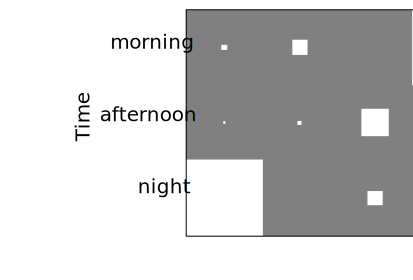
\includegraphics[width=0.6\textwidth]{images/absent_groundtruth.png}
\caption[Simulated object location ground truth distribution]{Simulated object location ground truth distribution.
The x-axis represents the locations the y axis represents the timezones. The size of the white box indicates the probability of the object presence.}
\label{absent-gt}
\end{figure}

From the ground truth we can observe that there is higher probability to find the object in the sink during night time and in the cabinet during the other time periods. We need to develop models which can learn these temporal patterns from the observations

\section{Evaluation}

\todo[inline]{TODO}

We compare the Dirichlet-Categorical-Bernoulli model with the Hierarchical-Dirichlet-Categorical model explained in \ref{sec: HDCM}. We compare the ground truth dirichlet probabilities, used to generate the simulated dataset and the learned probabilities and evaluate the performance of the learning. 
We use the adopted  Bhattacharyya distance \cite{rauber2008bhattacharyya} to quantify the similarity between the simulated and the learned Dirichlet distribution.
\begin{figure}
    \centering
    \includegraphics[width=\textwidth]{images/absent_learned.png}
       
    \begin{minipage}[t]{.35\textwidth}
    %\centering
    \subcaption{Ground Truth}\label{fig:absent-gt}
    \end{minipage}%
    \begin{minipage}[t]{.3\textwidth}
    %\centering
    \subcaption{HDC model}\label{fig:absent-hdcm}
    \end{minipage}
    \begin{minipage}[t]{.25\textwidth}
    %\centering
    \subcaption{HDCB model}\label{fig:absent-hdcmb}
    \end{minipage}

\caption[Model Evaluation of HDC and HDCB ]{Model Evaluation: \ref{fig:absent-gt} is ground truth of the distribution. \ref{fig:absent-hdcm} is the learned distribution using the HDC model. \ref{fig:absent-hdcmb} is the learned distribution using the HDCB  model }
        \label{fig:absent-eval}
    
\end{figure}


\begin{figure}[htp]
\centering
\includegraphics[width=\textwidth]{images/bhatta-distance.png}
\caption[Model evaluation : Bhattacharyya distance]{Bhattacharyya distance between the ground truth and the learned distributions for different size of training data. }
\label{}
\end{figure}




\documentclass[11pt]{book}
%Gummi|063|=)
\title{\textbf{Complete this book }}
\author{Deebul Nair}
\date{}

\usepackage{amsmath}
\usepackage{todonotes}

\usepackage{tikz}
\usepackage{amsmath}
\usetikzlibrary{bayesnet}
\usepackage{tabularx}

\begin{document}

\chapter{In-House Human Presence Model}

Domestic robots in future should be able to gather knowledge about the favourite places of the humans in the home and also the time period when they mostly occupy their favourite places. This acquired knowledge of the human presence patterns shall enable the robots to make better decisions. For example what time particular rooms are unoccupied for cleaning or when to turn on the heater of the room. 

In this chapter we focus on such knowledge accession from observations made by the robot. However, the advancement in long term autonomous navigation \todo{cite} and the rapid adoption of databases in the robots \todo{cite} has not only made it feasible for domestic robots to acquire such knowledge, but also a number of challenges.  In more details, these challenges are the (i) modelling human presence (ii) prediction of future location (iii) learning all these with sparse observations made by the robots. 

Significant progress has been made on a related problem by researchers in the field of human location behaviour, which is to learn the patterns in human location outdoors. Approaches for learning routine mobility  range from purely temporal (\cite{c1, c2}), spatial (\cite{c5,c3}), to a combination  of  both  (\cite{c4}). Non-parametric Bayesian methods are also gaining popularity given their ability to refine models as more data arrives. Chen et al. (2012) used a Gaussian process to model congestion on road networks, while Gao et al. (2012) used a hierarchical Pitman Yor process to model check-in behaviour on location-based social networks. Indoor human location behaviour was studied by \todo{cite}Krajnik et al.  using Fourier transform methods and Gaussian mixture models. 

while Krajnik's  work is first step towards learning human mobility behaviour in indoor environments, it failed to address the problem of sparse dataset in domestic robots. Observations made by the robots are very sparse. We aim to demonstrate in this chapter that, by using Bayesian models, we can capture the human behaviour patterns in a sparse dataset.




\begin{thebibliography}{99}

\bibitem{c1} J.  McInerney,  J.  Zheng,  A.  Rogers,  and  N.  R.  Jennings.Modelling heterogeneous location habits in human populations for location prediction under data sparsity. In Interna-tional Joint Conference on Pervasive andUbiquitous Com-puting (UbiComp 2013)
\bibitem{c2}  S.  Scellato,   M.  Musolesi,   C.  Mascolo,   V.  Latora,   and A.  Campbell. Nextplace:   a  spatio-temporal  prediction framework for pervasive systems.  InPervasive Computing
\bibitem{c3} L. Song, D. Kotz, R. Jain, and X. He.  Evaluating next-cell predictors with extensive wi-fi mobility data. IEEE Trans-actions on Mobile Computing , 5(12):1633–1649, 2006 pages 152–169, San Francisco, CA, USA, 2011. Springer.
\bibitem{c4}N. Eagle and A. S. Pentland.   Eigenbehaviors:  identifying structure in routine. Behavioral Ecology and Sociobiology ,63(7):1057–1066, 2009.
\bibitem{c5} H.  Gao,  J.  Tang,  and  H.  Liu.   Exploring  social-historical ties on location-based social networks.  In6th InternationalAAAI Conference on Weblogs and Social Media, 2012
\bibitem{c6} Krajnik, Tomas, Miroslav Kulich, Lenka Mudrova, Rares Ambrus, and Tom Duckett. “Where’s Waldo at Time T? Using Spatio-Temporal Models for Mobile Robot Search.” In Robotics and Automation (ICRA), 2015 IEEE International Conference on, 2140–2146.

\end{thebibliography}



\section{Aruba Dataset}
In our thesis we used a  publicly-available  dataset  Aruba published by the Lincoln Center for Autonomous Systems, LCAS \todo{cite \cite{STRANDS}}. The dataset is of person presence collected at a smart apartment by the Center for Advanced Studies in Adaptive Systems, CASAS \todo{cite \cite{STRANDS}}.

The testbed where the dataset was collected is a  three-bedroom apartment located on the Washington State University that is part of CASAS smart home project. 
\begin{figure}[htp]
\centering
\includegraphics[width=\textwidth]{images/aruba-flat.png}
\caption{Aruba apartment visualization}
\label{aruba}
\end{figure}
As shown in Figure \cite{aruba}, the smart apartment test bed includes three bedrooms, one bathroom, a kitchen, and a living / dining room.  The apartment is equipped with motion sensors distributed approximately 1 meter apart throughout the space. The Aruba dataset was extracted from these motion sensor dataset provided by CASAS. The dataset contains the location of a person in the apartment every minute for 16 weeks.

\subsection*{Sparsification}
Aruba dataset is a large dataset as compared to an person location dataset we assume the robot will be able to generate. The Aruba dataset has recordings of every minute for 118 days, which is 161280 readings.
On the contrary the assumed dataset which will be collected by the robot by autonomously roaming in a home will be just 3-5 readings per day.
So for simulating the sparsity in the object location dataset we will sparsify the ARUBA dataset by random selecting only selecting 3-5 readings each day.

\subsection*{Visualization}
We visualize the dataset to find out if as humans we can find any patterns in the data. Since the observations are of 2 dimension(location vs time) the visualization is feasible. As explained in the section \todo{cite the central thesis}, we try to learn daily patterns by dividing the data into per hour cycle. As visualized in Figure \cite{aruba-visual} we can find that there are some prominent patterns emerging which can be learned. For example the usage of the Bedroom, Living room, outside and kitchen.

\begin{figure}[htp]
\centering
\includegraphics[width=\textwidth]{images/aruba-data.png}
\caption{Aruba Dataset Visualization : The X -axis are the locations of the home, Y-axis are the hours of the day. The intensity of the color in each box indicates the number of times the person is present in that location. Higher the intensity means more time is spent by the person in that location at that time.}
\label{aruba-visual}
\end{figure}


\section{Dirichlet Categorical model }

Dirichlet Categorical model (DCM) is a 2 level Bayesian model. The basic idea is that observations of each time period is characterized by a distribution over the possible locations.

The data are the observed human location $x_{ij}$ for $i = 1 \dots T$ time periods and then $j = 1, \dots , N$  are the observations.  We assume that the latent pattern in the persons location per period are distributed as a categorical distribution. The number of periods $T$ for our model is fixed to 24 corresponding to the number of hours in a day. 

The Dirichlet-Categorical model is the generalization of the Beta-Binomial model to multiple classes of a categorical or multinomial distribution. The conjugate prior for the categorical distribution is the Dirichlet distribution. The model estimates the posterior distribution of $\theta_i$ given our current data and prior beliefs. Our prior beliefs are encoded in the model through the hyperparameter $\alpha$, which represents pseudocounts of what we believe the data should look like – typically set as 1's for weak uniform beliefs. The graphical diagram of the model is shown in Figure \cite{dcm}

\noindent
\begin{figure}[htp]

\begin{minipage}{0.3\textwidth}
\centering

\tikz {
\node [const]                  (alpha) {$\alpha$};
\node [below=of alpha, latent]  (theta) {$\theta_i$};
\node [below=of theta, obs]     (x)     {$x_{ij}$};
\edge {alpha} {theta};
\edge {theta} {x};
\plate {trials} {(x)} {j data};
\plate {bags} {(theta)(x)(trials)} {i time};
}

\end{minipage}%
\begin{minipage}{0.7\textwidth}

\begin{equation*}
	\alpha = <1, 1, .... , 1 > 
\end{equation*}
\begin{equation*}
	\theta_i  \sim Dirichlet(\alpha)
\end{equation*}
\begin{equation*}
	x_{ij} \sim Categorical(\theta_i)
\end{equation*}
\end{minipage}
\caption{Graphical model representation of DCM. The boxes are ``plates" representing replicates. The outer plates represents hours of a day, while the inner plate represents the choice of places within each hour.}
\label{dcm}
\end{figure}



\section{Explanation : From LDA}
All the models in the thesis are based on the ``bag of words" assumption-- that the order of the data in a day can be neglected.
In language of probability theory, this is an assumption of \emph{exchangeability} for the words in the document (Aldous, 1985)

from : http://blog.nullspace.io/motivating-bayesian.html
an important class of models called exchangeable models are guaranteed by de Finetti’s theorem to decompose cleanly into the definition of the Bayesian framework.

One reason exchangeability is interesting is because prima facie, although it seems to be similar to the assumption of iid, it is actually much richer, and much less restrictive. Consider, for example, if we have a document whose words have been shuffled. Intuitively, if we see an Arabic word, then even it is much more likely that we will encounter other Arabic words elsewhere in the document, since there is a reasonable probability the document itself is in Arabic. The assumption of iid does not capture this, because the words are assumed to be completely independent. Exchangeability doesn’t assume independence, however, only that ordering doesn’t matter, so this will be captured in a model that is exchangeable.

This is a critical aspect of Bayesian inference that many people simply don’t understand, and it has all sorts of consequences, like making Bayesian nonparametrics possible, and making conditional probabilities uncomputable in general. It is so convenient to think of this class of problems as Bayesian that it seems like a crime to not use Bayesian inference.


\begin{itemize}
	\item Generative probabilistic model
	\item three-level hierarchical Bayesian model
	\item 
\end{itemize}


\section{Discussions}

http://andrewgelman.com/2016/08/22/bayesian-inference-completely-solves-the-multiple-comparisons-problem/
http://andrewgelman.com/2013/11/21/hidden-dangers-noninformative-priors/

The point of the story in that slide is that flat priors consistently give bad inferences. Or, to put it another way, the routine use of flat priors results in poor frequency properties in realistic settings where studies are noisy and effect sizes are small.
\label{sec:}

% section  (end)
\end{document}



\chapter{Learning Room Occupancy based on User Routines}
\label{chapter:occupancy}
In this chapter, we investigate how a robot can learn occupancy period of different rooms of a office or home based on user's routine. Occupancy represents the belief of the robot about when are rooms occupied or empty. The probabilistic model developed in the previous chapter enables a domestic service robot to learn the user preference for object placement on each locations. We use the same models in this chapter to learn about the occupancy of each rooms

We consider the example of a cleaning robot which needs to decide what time of the day is best suited for cleaning. \cite{Fink2013} did a exhaustive survey about usage, adoption process and long-term effects of domestic cleaning robot in people's homes. One of the biggest barrier for better adoption of robots in household was compatibility with habits and routines. Thus in order for a robot to clean a house or office with minimum intervention, it should have the ability to fully understand its user routines, to make decisions based on the state of each rooms. Thus if the robots can learn the  least occupancy time of the environment it can make decisions on cleaning time which will cause minimum interference for humans. 


In this chapter the robot will learn multiple user's routine in using different rooms of a office and determine the low occupancy time for cleaning.
The robot might use a camera sensor and standard person detection algorithm to detect the human. This generated information are recorded by the robot in its robot memory along with the time and room of the observations. We develop a Bayesian model which can learn from these observations and generate the occupancy periods for each room. In particular, our approach allows a robot (1) to infer the occupancy time of each room (2) to make predictions about future occupancy of each rooms. In our experiments, we demonstrate that robots with our models can learn and predict accurately if a room is occupied.

In the next section we will explain the model used to learn the occupancy periods of each rooms. 

\section{Hierarchical Beta Bernoulli Model}

Hierarchical Beta Bernoulli model explained in Chapter~\ref{chapter: object} is also used to model the occupancy of each room. In Chapter~\ref{chapter: object} the observation were boolean values representing the presence of an object at a particular location. The observations here is also a boolean value representing if the room is occupied. From these boolean observations we need to learn the latent knowledge about the occupancy, and we use the Bernoulli distribution to represent these observations, while the latent occupancy of the room is represented by the Beta distribution. 
Now the model learns the latent knowledge about the occupancy separately for each hour of the day. To enable sharing of knowledge between different times of the day we use the third level of the model, which forms the conjugate prior for the Beta distribution. These ensure the knowledge about latent factor in 1 time period are shared with other time periods. 

\noindent
\begin{figure}[htp]

\begin{minipage}{0.3\textwidth}
\centering

\tikz {
 % Define nodes
  \node[latent]                                 (theta) {$\theta$};
  \node[latent, above=of theta, xshift=-1.2cm]  (alpha) {$\alpha$};
  \node[latent, above=of theta, xshift=1.2cm]   (beta) {$\beta$};
  \node[obs, below=of theta]                    (y)     {$x$}; 
  % Connect the nodes
  \edge {alpha,beta} {theta} ; %
  \edge {theta} {y};
  % plates
  \plate {location} {(y)} {location};
  \plate {time} {(theta)(y)(location)} {time};
}

\end{minipage}%
\begin{minipage}{0.7\textwidth}

\begin{equation*}
	\alpha \sim Beta(2,2) ; \beta \sim Beta(2, 2);
\end{equation*}
\begin{equation*}
	\theta \sim Beta(\alpha, \beta);
\end{equation*}
\begin{equation*}
	x = Bernoulli(\theta)
\end{equation*}
\end{minipage}
\caption[Hierarchical Beta Bernoulli graphical model]{Graphical model representation of Hierarchical Beta Bernoulli model. The boxes are ``plates" representing replicates. The outer plates represents hours of a day, while the inner plate represents if the room has users in that hour.}
\label{bbm2}
\end{figure}



The model can be explained as:

	\boldmath{$\alpha$} and \boldmath{$\beta$} is  prior beta distribution, 
	
	$\theta_i$ is the latent occupancy distribution for period $i$  ,
	
	$x_{ij}$ is the observation in period $i$.


\begin{figure}
    \centering
    \begin{subfigure}[b]{0.21\textwidth}
        \includegraphics[width=\textwidth]{images/scitos.jpg}
        \caption{}
        \label{fig:scitos-1}
    \end{subfigure}
    ~ %add desired spacing between images, e. g. ~, \quad, \qquad, \hfill etc. 
      %(or a blank line to force the subfigure onto a new line)
    \begin{subfigure}[b]{0.6\textwidth}
        \includegraphics[width=\textwidth]{images/kth-dataset-2.png}
        \caption{}
        \label{fig:robot-view-1}
    \end{subfigure}
    \caption[Brayford dataset collection]{Brayford Dataset collection: SCITOS-G5\footnotemark Robot used for data collection \ref{fig:scitos-1} \protect. Images \footnotemark as seen by the robot at the different rooms in the lab \ref{fig:robot-view-1}}\label{fig:brayford-dataset}
\end{figure}

\footnotetext{\url{ http://www.hanheide.net/2013/06/brand-new-robot.html}}
\footnotetext{\url{https://www.youtube.com/watch?v=aTr9KD4XMGc }}


\section{Experiments}
We conducted our experiments on real data collected by a robot in an office environment. The robot for each room in the office makes observation of its occupancy. The goal of the experiment was to verify that
\begin{itemize}
    \item the robot is able to learn the room occupancy probability.
	\item the resulting model allows for accurate prediction or future occupancy of the room
\end{itemize}

\subsection{Evaluation of Model accuracy}

We evaluated the model accuracy using cross-validation methods on the Brayford dataset. Brayford dataset is extracted from the Witham Wharf RGB-D dataset, both collected as part of the Spatio-Temporal Representations and Activities for Cognitive Control in Long-Term Scenarios (STRANDS) project. 
Witham Wharf RGB-D dataset is used for testing RGB-D localization in changing environments. The dataset consist of RGB-D images collected over eight locations in an open-plan office. The Brayford dataset was extracted from the above dataset by manually annotating the presence of human in the room at the moment. Figure~\ref{fig:brayford-dataset} shows the data collection method. Data was collected using the SCITOS-G5 robot. 



\begin{figure}[htp]
\centering
\includegraphics[width=\textwidth]{images/occupancy_hist_withresults.png}
\caption[Brayford Dataset ]{Brayford Dataset: normalized human occupancy per hour per room. The shaded regions are the learned cleaning time period for each room.}
\label{fig:brayford_visualization}
\end{figure}

\FloatBarrier



The dataset is divided in 2 parts the training set and testing set. The training set consist of 7 days of observations, where the robot visits predefined eight locations of the office at a regular interval of 10 minutes each. The testing set consist of another week of observation. Figure~\ref{fig:brayford_visualization} is the bar plot of the observations made by the robot. 



The training dataset was used to learn the parameters of the model while the testing dataset was used to predict and validate the learned models. 
The accuracy results of the 8 rooms is plotted in Figure~\ref{fig:brayford_evaluation} . The model predicts with above \textbf{80\%} accuracy for 3 rooms kitchen, resting area and workplace04 . While accuracy of predictions for other rooms are in the range of 60\% to 80\% .

\begin{figure}[htp]
\centering
\includegraphics[width=0.7\textwidth]{images/Brayford_dataset_results_evaluation.png}
\caption[Brayford Dataset Evaluation]{Brayford dataset evaluation: Accuracy of the model for different rooms in the office}
\label{fig:brayford_evaluation}
\end{figure}



Based on the learned occupancy parameter for each room, the robot can now determine which are the period of low occupancy and select these time periods for doing its cleaning task. The shaded region in the Figure~\ref{fig:brayford_visualization} are the learned time periods in which the robot can perform cleaning task.
\FloatBarrier

\section{Discussions}

In this chapter, we presented a probabilistic framework for learning the occupancy periods of each rooms. The robot continuously records in its robot memory when and where it saw the users. Now based on the data collected the robot now does an analysis gain knowledge about the occupancy of each room. 

We have used the identical model as discussed in chapter ~\ref{chapter: object} for learning the occupancy parameter. This demonstrates the flexibility of the probabilistic programming in which we can reuse the models to new problems.
From the experiments conducted on real world datasets collected by mobile robots in an open office we can conclude that the model is able to learn accurately the latent occupancy time periods. 

\chapter{Knowledge-enabled fault tolerant object search}
\label{cha}

Efficient searching for objects in the environment is one of the application for the knowledge being learned from object locations. The learned knowledge is as heuristics to improve the search time of objects. There are 2 basic methods in which we can use the learned knowledge as heuristics, first we can search for objects in the decreasing order of the learned probabilities or alternatively we can use the descriptive model to predict based on its learned probabilities. However the probabilistic representation of the learned knowledge can be used in ingenious way to solve more complex problems. Markov Decision Process (MDP) based planners can use the learned probabilities in their decision process to make more informed decisions. To illustrate this flexibility we have used the learned probabilities to make a sequential decision search algorithm which can accommodate the recognition failure in the vision algorithms.
\missingfigure{Image with false detection}
Household robots need to be able to recognize the objects they’re supposed to search and manipulate. But while object recognition is one of the most widely studied topics in artificial intelligence, even the best object detectors still fail much of the time. As a result there are very much possibilities that even though the search algorithm has provided the correct location the object detector might fail to locate the object. An alternative will be provide a search algorithm which can accommodate the object detector failures. All these object detectors along with the detection also publish the confidence(probability) of the detection. The proposed algorithm here combines both the \emph{detection probability} and the \emph{learned probability} of the objects and provide sequential decisions for the next location to search.

\section{Search as a decision Framework}
\todo[inline, caption={search1}]{Introduce the topic name}
\todo[inline, caption={search2}]{Add the 2 papers as the related work of probabilistic search in robotics}
\todo[inline, caption={search3}]{ and that the below model is a reduced version and simplified model}

The  contributions  of  this  paper  include  the  formulation of the search control problem as a decision-making problem rather  than  a  sensing  task,  where  measures  associated  with decisions,  e.g.  confidence  and  robustness  of  the  decision or  time  until  the  decision  is  made,  are  used  to  design  an appropriate  control  policy.  Our  formulation  of  the  search problem  as  a  detection  problem  also  allows  us  to  include practical  sensor  artifacts  (such  as  false  alarms  and  missed detections)  which  have  not  be  completely  considered  in other  formulations  [6]  of  the  search  problem.


A Decision-Making Framework for Control Strategies
in Probabilistic Search
Timothy H. Chung and Joel W. Burdick

A probabilistic framework for object
search with 6-DOF pose estimation 
\todo[inline]{robotics search in robots as POMDP in its related work}
\section{Model}
The idea is use the learned knowledge of the object locations as the first guess (prior ) of the probabilities that the object in question is located in each of the possible object locations. The prior probabilities suggest which location to search first. If the object is not found in that location, the prior probabilities are then updated (yielding the posterior), and the process is repeated until the object is found. 

Assume that the domain of interest is a home we call $D_s$, which is made up of n spatial areas. Let $Y_i = 1$ if the object is in the \emph{i}th location, and then $Y_i = 0$ if it is not; $ i = 1, .... , n$. Now as discussed above object detectors can fail to detect the object. So, let $Z_i = 1$ if the object is found in the \emph{i}th location, and $Z_i = 0$ if not.

We can define two terms \emph{detection probability},
\begin{equation}
	p_i = Pr(Z_i = 1| Y_i =1), \qquad  i = 1,...,n,
\end{equation}
which is a conditional probability, and the \emph{occurrence probability},
\begin{equation}
	\pi_i = Pr(Y_i = 1),\qquad  i = 1, .... , n.
\end{equation}

This can be expressed in probabilistic programming form:
\begin{gather}
	Z_i | Y_i \sim Bernoulli (Y_i, p_i), \qquad  i  = 1,....,n \\
	Y_i \sim Bernoulli(\pi_i),\qquad   i = 1,...,n,
\end{gather}

where, the occurrence probability {$\pi_i$} is given by the learned probabilities, while the detection probability {$\pi_i$} is provided by the object detector algorithm.

Now, assume that hte \emph{i}th location is searched by the robot and the object is not found (i.e., $Z_i = 0$). In that case, the probability that the object is in the \emph{i}th location is updated using Bayes' Theorem. This yields the posterior probability,

\begin{align*}
	Pr(Y_i = 1 | Z_i = 0) &= \frac{Pr(Z_i = 0|Y_i=1)Pr(Y_i=1)} {Pr(Z_i=0)} \\
	                       &= \frac{Pr(Z_i = 0| Y_i =1 )Pr(Y_i =1)}{Pr(Z_i=0|Y_i =1)Pr(Y_i = 1) + Pr(Z_i=0|Y_i=0)Pr(Y_i=0)} \\
	                       &= \frac{(1 - p_i)\pi_i}{(1 - p_i)\pi_i + (1)(1 - \pi_i)} \\
	                       &= \frac{(1 - p_i)\pi_i}{1 - p_i\pi_i}
\end{align*}

where we assume that there are no false-positive detection (i.e., $Pr(Z_i =0| Y_i = 0) = 1$). Note that the new posterior is less than the prior probability $\pi_i$ as the object was not observed.

Since the object is not found in the searched location, then this should also affect the posterior probability in the other grid boxes. For example, consider the \emph{j}th location, where $j \neq i$. Then,
\begin{align*}
	Pr(Y_j = 1 | Z_i=0) &= \frac{Pr(Z_i = 0 | Y_j = 1)Pr(Y_j = 1)}{Pr(Z_i = 0)} \\
	                    &= \frac{\pi_j}{ 1 - p_i\pi_i}
\end{align*}

Thus, the posterior probability of the object being the \emph{j}th location is greater than the prior probability $\pi_j$ . These new posteriors will then become the next prior probabilities is a sequential procedure that would determine the next location to search.

\section{Example}
\todo{split as 2 example , 1 with high detection probablity 0.9 and other with 0.6}
\todo{show the different sequence}
Suppose we have a domestic robot which has learned the location probabilities of a cup in a home. The robot has learned that the cup can be found 3 locations in the home, thus the domain for search can be defined as $D_s = \{cupboard, table, dishwasher \}$ . 
Now lets assume the robot has been in the room for long enough and made some observations. Based on these observations it learns the occurrence probabilities as $p_i = \{ 0.8, 0.1, 0.1\}$ . The object detector for the cup has a \emph{detection probability} of $p_{cup} =  0.6$ .

As you can see there is a strong probability of finding the cup in the cupboard. The algorithm selects to search the cupboard. But the object detector fails and is not able to detect the cup. If we are not using the algorithm the robot will move on to the next location to search the cup in the next location.


\missingfigure{Illustration of the proabbiliities and how they change with each observation}

However our algorithm on the failure detection will update its probabilities and the updated posterior probability will be $ p_i = \{ 0.44, 0.27, 0.27\}$ and it still selects to search the cupboard for the next time. This illustrates the algorithm understands the limitation in the object detector and updates its beliefs to accommodate this limitation and make better \emph{informed} decisions.  

 
\section{Evaluation}
hey you didnt think about evaluation ? 
% chapter  (end)
\chapter{Integration with FAWKES framework}
\label{cha:}

% chapter  (end)

\chapter{Conclusions}
\label{cha:}


We believe as and as robots become more autonomous, the robot will be able to record more and more obserations. This will help the approaches discussed in the thesis to be more accurate and make better predictions.
\section{Future Work}


% chapter  (end)
% bibliography and appendixes
\include{bibliography}
\begin{appendices}
	
\chapter{Bhattacharyya distance}
	 The Bhattacharyya distance\cite{bhattachayya1943measure} is a measure of divergence between
probability distributions, that allows measuring the dissimilarity between two continuous or discrete probability distributions. It can take values from 0-$\inf$. The value is 0 when both the distributions are similar and $\inf$ when there is no overlap between the distributions. Adopting the  Bhattacharya distance to Dirichlet distributions \cite{rauber2008bhattacharyya} we get :
\begin{multline}
	D_B(Dir_a(x_1, \dots ,x+n), Dir(y_1, \dots , y_n)) = \nonumber\\
	 \Gamma \Bigg( \frac{1}{2}  \sum_{i \in {1, \dots, n}} x_i +  \frac{1}{2}\sum_{i \in {1, \dots, n}} y_i\Bigg) + 
	\frac{1}{2}  \sum_{i \in {1, \dots, n}} \Gamma (x_i) + 
	\frac{1}{2}  \sum_{i \in {1, \dots, n}} \Gamma (y_i) - \\ 
	\sum_{i \in {1, \dots, n}} \Gamma \bigg(\frac{1}{2} (x_i + y_i) \bigg) - \frac{1}{2}  \Gamma \Bigg(  \sum_{i \in {1, \dots, n}} x_i \Bigg) + \frac{1}{2}  \Gamma \Bigg( \sum_{i \in {1, \dots, n}} y_i\Bigg)
\end{multline}


\end{appendices} 


%\emptypage
%\emptypage

\end{document}
